\documentclass{standalone}

\usepackage{graphics}
\usepackage[dvipsnames,svgnames]{xcolor}

\usepackage{tikz,pgf,pgfplots,circuitikz}
\pgfplotsset{compat=1.15}
\usetikzlibrary{intersections,arrows.meta,angles,calc,3d,decorations.pathmorphing}
\usepackage[compat=1.1.0]{tikz-feynhand}

\usepackage{amssymb,amsfonts,amsthm,mathtools}
\usepackage{physics,braket,bm}

\begin{document}  
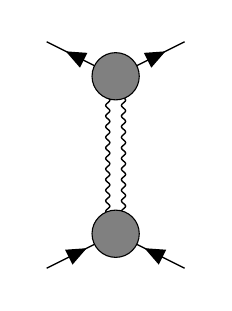
\begin{tikzpicture}[baseline=(o.base)]
  \begin{feynhand}
    \vertex (o) at (0,0) {};
    \vertex (p1) at (-1,1.5) {};
    \vertex (p2) at (1,1.5) {};
    \vertex (p3) at (-1,-1.5) {};
    \vertex (p4) at (1,-1.5) {};
    \vertex (o1r) at (0.1,1){};
    \vertex (o1l) at (-0.1,1){};
    \vertex (o2r) at (0.1,-1){};
    \vertex (o2l) at (-0.1,-1){};
    \propag[boson] (o1r) to (o2r);
    \propag[boson] (o1l) to (o2l);
    \vertex (o1) at (0,1){};
    \vertex (o2) at (0,-1){};
    \propag[fermion] (o1) to (p1);
    \propag[fermion] (o1) to (p2);
    \propag[fermion] (p3) to (o2);
    \propag[fermion] (p4) to (o2);
    \filldraw[fill=gray, draw=black] (o1) circle [radius=0.30cm];
    \filldraw[fill=gray, draw=black] (o2) circle [radius=0.30cm];
  \end{feynhand}
\end{tikzpicture}
\end{document}
